\versoimage
\chapter{TLS Identification In \lin{3D}}\label{ch:threedee}
\loftchap{TLS Identification In \lin{3D}}
\chapterprecis{That's some fancy lookin' graphs you got there.}

\section{Dump from Sci Rep}
Decoherence sources such as the environmental two-level system (TLS)~\cite{Dutta1981, Shnirman2005} are presently a major hurdle to the realisation of operational superconducting qubits and other Josephson junction based quantum devices.
Many properties of the TLS have been probed experimentally, demonstrating relatively long decoherence times whilst showing them to be stable and controllable~\cite{Simmonds2004, Neeley2008, Shalibo2010, Lupascu2009, Lisenfeld2010}.
However, identifying their true microscopic nature remains an open problem. Controllable superconducting qubit architectures (charge, flux and phase) make it possible to study single `strongly coupled' TLSs~\cite{Neeley2008, Lupascu2009, Lisenfeld2010}, as opposed to weakly coupled ensembles of TLSs that may be responsible for $1/f$ noise~\cite{Dutta1981,Schriefl2006}.
Although the Standard Tunneling Model (STM) \cite{Anderson1972, Phillips1972} can be used to explain all existing experimental results, to improve devices we need detailed a microscopic understanding of these defects.

Many microscopic models have now been proposed: delocalised oxygens~\cite{DuBois2013,DuBois2015}, surface state interactions~\cite{Choi2009,Lee2014}, polaron dressed electrons~\cite{Agarwal2013} and alien species (primarily hydrogen)~\cite{Jameson2011, Holder2013, Gordon2014}; all of which are possible decoherence sources and/or explain the origin of strongly coupled TLSs.
Better fabrication methods, higher vacuums and more robust qubit designs have historically suppressed or diminished the response of such noise sources~\cite{Vion2002, Martinis2005, Koch2007, Schreier2008, Houck2008}.
However, continuing down the path of a perfectly clean but amorphous dielectric may no longer be the optimal direction. Whilst crystalline layers are difficult to construct in this environment, they are possible and show a dramatic decrease (of up to 80\%) in visible TLSs over their amorphous counterparts~\cite{Oh2006}.

Such a decrease could be explained via our previous work on the delocalised oxygen model~\cite{DuBois2013,DuBois2015}, where we suggest the origin of some TLS defects are oxygen atoms in a spatially delocalised state due to the non-crystalline nature of the dielectric layer.
As such, this is a concrete microscopic ensemble of the classic atomic tunneling model: typically cited as motivation for the STM (which is more general, as the tunneling object need not be a single atom).

This model discussed a simplified configuration space using low dimensional arguments, culminating in a \lin{2+1D} framework where a cage of six aluminium atoms surrounded a central oxygen atom in three dimensions and calculated observations based on the oxygen delocalising on a two dimensional plane.
The dimensional simplicity of this model allowed a direct matrix diagonalisation approach to solve a time independent Schrödinger equation, which due to memory limits could not be extended into a complete \lin{3D} representation of a TLS defect.

Here we introduce an alternative method to this model which can obtain a complete three dimensional picture of the delocalised oxygen ground and excited states.
As the work in this report is a higher dimensional extension of the \lin{2+1D} model, its terminology has been retained herein.
It is suggested the reader be familiar with the discussions in \onlinecite{DuBois2015}, although a short summary of the nomenclature is outlined below.
Using this more powerful technique, we are able to move beyond a simplistic cubic representation and investigate true lattice configurations and realistic amorphous positions from our DFT studies~\cite{DuBois2013,DuBois2015a}.

Two defect types are investigated, both of which stem from deforming the crystalline lattice of corundum: the low temperature and pressure phase of $\ce{Al_2O_3}$ (the  closest Al--O bond distance in this phase is $\sim\!1.85$ \AA).
Defect type A; where the aluminium--oxygen bond distance is shortened, forcing the oxygen to occupy one of two off-axis positions, and defect type B; where the opposite occurs: the aluminium--oxygen bond distance is lengthened, allowing two preferred oxygen positions, on-axis.

The trigonal lattice structure of this crystalline material and the amorphous nature of a JJ barrier give rise to many complications for a microscopic model, due to potential contributions from many neighbouring atoms to a possible defect site.
Therefore, to fully understand the response to these interactions, we start with a very simplistic cluster of atoms and add complexity once an understanding of rudimentary exchanges is achieved.

Defining the oxygen position to be at an origin, two introduced aluminium atoms can be considered as pairs ($x = -X, \: +X$ = \{$\pm 1.85$ \AA\}) lying on a cardinal axes; which are identified as $\abs{X}$ or simply referred to as the `defect pair'.
Displacing $\abs{X}$ equidistantly from this origin (\ie moving away from optimal crystalline configuration) will yield either an A or B type defect, depending on the direction of displacement.
$\abs{Y}$ and $\abs{Z}$ describe aluminum pairs in the $y$ and $z$ directions respectively.

Eigenenergies of a system are frequently discussed in a relative fashion using a convention where $E_{ij} = E_j-E_i$, such that the ground state ($E_0$) to first excited state ($E_1$) energy splitting is defined as $E_{01}$.

\section{Results}

The capability to investigate oxygen delocalisation in \lin{3D}, using realistic atomic positions within an amorphous layer of $\ce{Al_2O_3}$ generates an extensive state space.
Hence we start the investigation using a simple three atom system comprising of an oxygen atom and a confining aluminium pair: $\abs{X}$.
An eigenspectrum is generated by increasing or decreasing the pair separation distance from the corrundum lattice distance $1.85$ \AA\ using the ground and five lowest excited energy levels of this system, depicted in \cref{fig:spect3d} (for comparison with the \lin{2D} model, see Figure 2 in \onlinecite{DuBois2015}).

\begin{figure}[htp]
  \resizebox{0.9\textwidth}{!}{\includestandalone{figures/spect3d}}
  \caption[Eigenspectrum]{\label{fig:spect3d}Eigenspectrum of a three atom system Al--O--Al, over a varying distance separation. Each excited state has been normalised with the ground state, which shows a clear $E_{01}$ degeneracy at large separation distance - indicative of a B type defect. An intermediate region exists as the separation distance decreases, which is approximately centered about the optimal Al--O bond distance of corundum ($1.85$ \AA). At small separation distances, the eigenspectrum is distributed over comparatively small energy levels, but is not degenerate (see \cref{fig:lift}).}
\end{figure}

In this figure an (an)harmonic division about $\abs{X} \sim 1.85$ \AA\ separates two regions with dissimilar properties.
In the region where $\abs{X} > 1.95$ \AA, a degenerate $E_{01}$ is observed and as the separation distance has increased, can be identified as a possible B type defect.
The second region ($\abs{X} < 1.55$ \AA) has a tightly bound eigenspectrum compared to the rest of the map although this yields no degeneracy.

In three dimensions, the potential minima manifests as a sphere around the location of an atom. As a consequence the three atom Al--O--Al chain produces a unique, rotationally symmetric ground state which is reminiscent of an oxygen interstitial defect in crystalline germanium~\cite{Artacho1995} and depicted in \cref{fig:lift}a\&b.\xxx{May need an override for this case too}
Comparatively, this region in the \lin{2D} case indicated the presence of an A type defect, as the \lin{2D} potential minima ring would be projected onto a plane, collapsing a degree of freedom.

Two other observations concerning the \lin{2D} to \lin{3D} transition is the dramatically reduced total energy values as wavefunctions are no longer artificially confined, and the higher excited states in the B type region now exhibit a quad degeneracy rather than two split doubly degenerate pairs---again because states are not artificially confined in the extra dimension.

\begin{figure}[htb]
  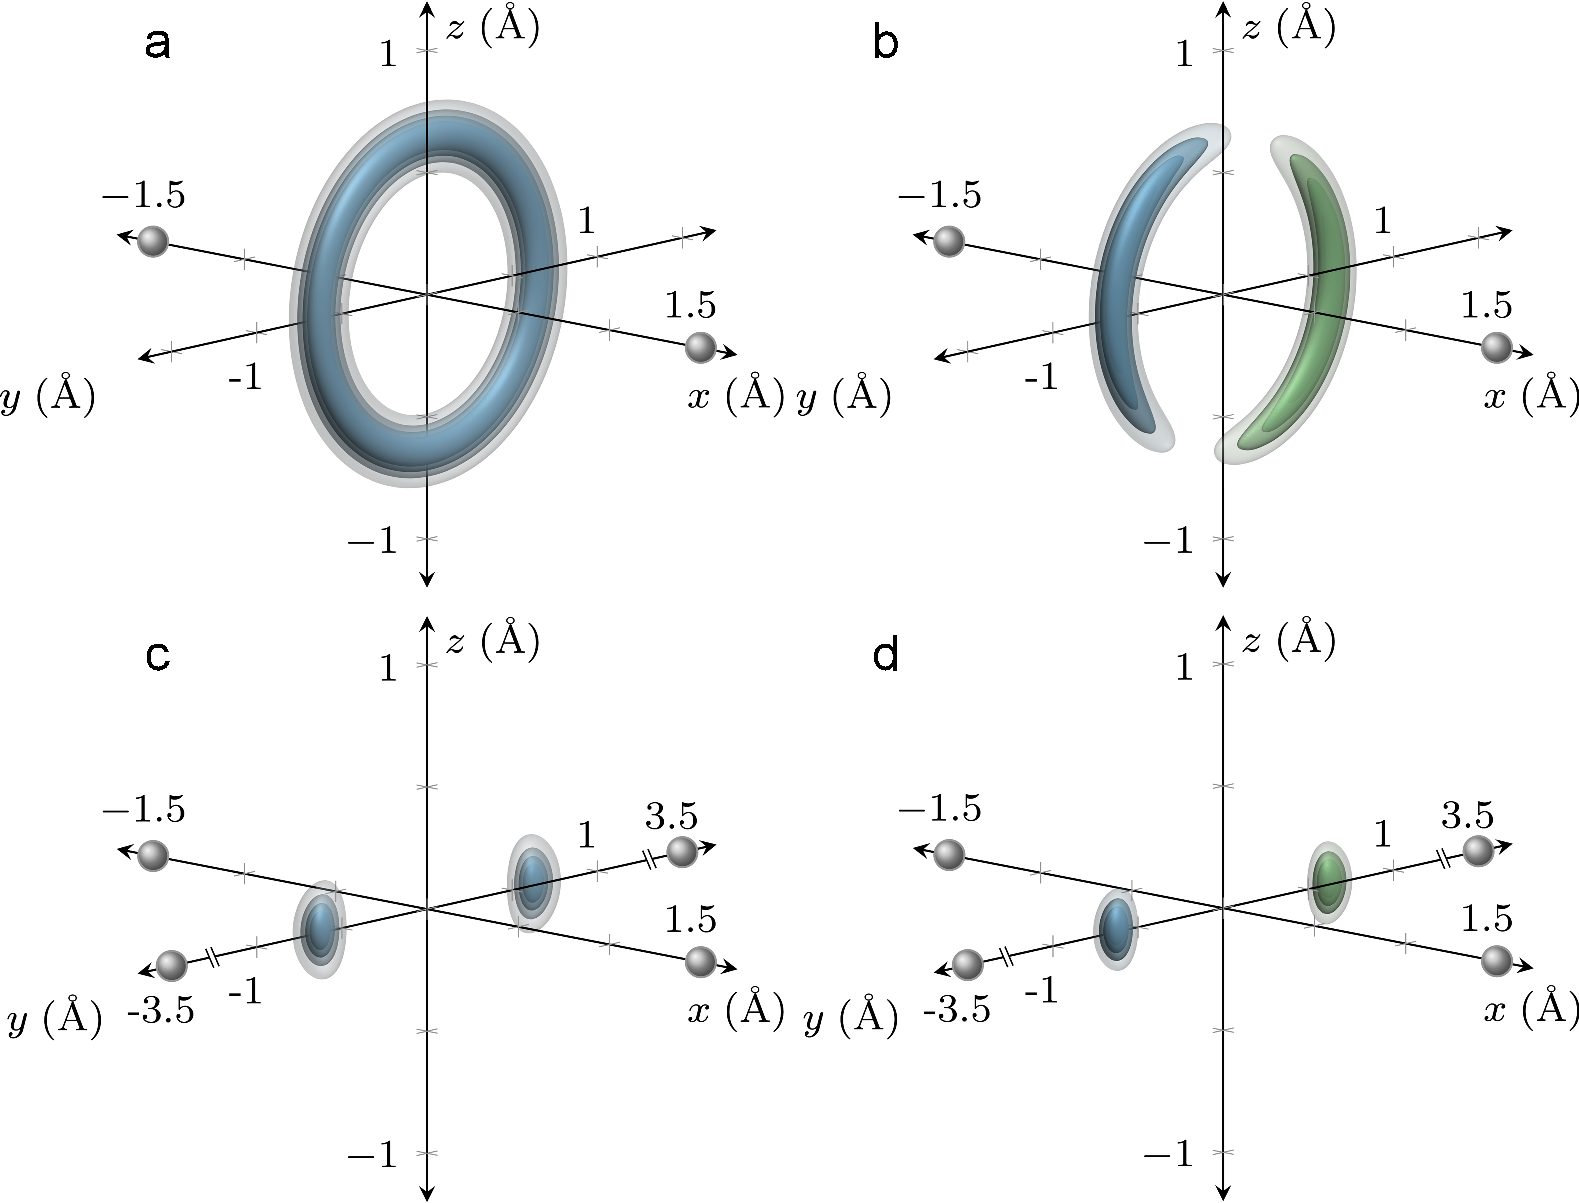
\includegraphics[width=\textwidth]{figures/lift}
  \caption[ground]{\label{fig:lift}Ground (left) and first excited (right) state wavefunctions of an Al--O--Al chain with $\abs{X} = 1.5$ \AA (aluminium atoms are depicted as gray spheres). Top axes show a unique ground state, the $E_{12}$ pair is degenerate in this case. Two more aluminium atoms are introduced at $\abs{Y} = 3.5$ \AA\ on the bottom axes, which causes degeneracy in the $E_{01}$ pair.}
\end{figure}

This simplistic three atom description can now be built upon to understand the interactions of a delocalised oxygen in a three dimensional space.
A confining pair is introduced in an additional dimension to the configuration in \Cref{fig:lift}a\&b, and the unique ground state is lifted to a degenerate $E_{01}$ pair; observing an A type TLS defect.
\Cref{fig:lift}c\&d illustrate this effect with a confining pair $\abs{Y} = 3.5$ \AA.
This distance is an arbitrary choice, as the shift occurs even at the cut-off limits imposed by the potential portion of the model~\cite{Streitz1994} (see \cref{sec:methods}).
In other words, any additional potential contribution which does not share the axial symmetry of the Al--O--Al chain will lift the degeneracy and result in a TLS.

\subsection{Oxygenic Orbitals}

A complete picture of the ground and excited state wavefunctions in \lin{3D} is now possible, which allows us to further investigate the properties of the two-level system and illustrate the importance of crystalline dielectrics in future Josephson junction devices.

A confined harmonic state can exist with many atomic configurations, and as with the low dimensional model, setting variables symmetrically is one of these cases.
\Cref{fig:lineharm} depicts the four lowest energy wavefunctions of an oxygen with six confining aluminium atoms: $\abs{X}\!=\!\abs{Y}\!=\!\abs{Z} = 1.6$ \AA.
Here the oxygen atom has no additional local minima to occupy, identifying this configuration as spatially localised, the harmonic approximation holds and the system is not considered as a TLS candidate.

\begin{figure}[htb]
  \resizebox{\textwidth}{!}{\includestandalone{figures/harmlike}}
  \caption[wfns]{\label{fig:lineharm}Wavefunctions of an oxygen confined by six equidistant aluminium atoms at $\abs{X}\!=\!\abs{Y}\!=\!\abs{Z} = 1.6$ \AA. This configuration exhibits a unique ground state (as shown in the energy level diagram) and hence is considered to be spatially localised.}
\end{figure}

From this localised case, we extend the $\abs{Y}$ confinement out to $2.1$ \AA.
Using the \cref{fig:spect3d} eigenspectrum we can predict this configuration to be a B type defect; where the $\abs{Y}$ separation distance is increased, and an oxygen dipole forms parallel to the $y$ axis.
This is indeed the case as shown in \cref{fig:lineb}.

\begin{figure}[htb]
  \resizebox{\textwidth}{!}{\includestandalone{figures/btype3d}}
  \caption[wfns2]{\label{fig:lineb}Wavefunctions of an oxygen confined by six aluminium atoms, where the symmetry of \cref{fig:lineharm} has been broken. $\abs{X}\!=\!\abs{Z} = 1.6, \abs{Y} = 2.1$ \AA, which manifests as a B type defect.}
\end{figure}

A particularly complex phenomenon emerged from the low dimensional model: quad degenerate ground states, where the energy difference between two degenerate pairs $E_{01}$ and $E_{23}$ approach the difference of the pairs themselves, \ie $E_{01} = E_{23} \approx E_{12}$.
\Cref{fig:linequad} shows a configuration expressing this behaviour.

\begin{figure}[tbh]
  \resizebox{\textwidth}{!}{\includestandalone{figures/quadwfn}}
  \caption[wfns3]{\label{fig:linequad}Wavefunctions of an oxygen confined by six aluminium atoms, where the confinement configuration is studiously pathological. $\abs{X} = 1.6, \abs{Y} = 2.1, \abs{Z} = 2.0$ \AA, yielding a quad degeneracy in the ground state due to the $E_{12}$ splitting existing below the superconducting gap ($\sim\! 100$ GHz, see text).  }
\end{figure}

The discussion in \onlinecite{DuBois2015} indicated that this form of degeneracy has a low probability of occurrence compared to A or B type defects.
Additionally, if $E_{12} \geq 100$ GHz the higher states ($E_{2}$ and $E_{3}$) can be ignored completely as energies of this magnitude dissociate Cooper-pairs, hence can be viewed as an operational upper bound for Josephson junction devices.
Splitting energies in \lin{3D} are much smaller than the \lin{2+1D} case, which suggests that the probability of these defects being experimentally visible may be higher than predicted with the low dimensional model based solely on this measure.
However, a comprehensive analysis of the three dimensional configuration space would need to be undertaken before real estimates of this behaviour can be given.

\subsection{A type defects and dipole considerations}

Whilst adding additional confinement pairs causes the unique, rotationally symmetric ground state of $\abs{X} < 1.55$ \AA\ (\cref{fig:lift}a\&b) to become degenerate; the third dimension yields a complication in the dipole measurement for the A type region.

Consider a system with parameters $\abs{X} = 1.53, \abs{Y} = 1.97, \abs{Z} = 1.95$ \AA, illustrated in \cref{fig:atypey}.
This system exhibits TLS behaviour, with $E_{01} = 40.63$ MHz, and a dipole strength in $y$ of $0.26 \; e$\AA: perpendicular to the confining $x$ axis as expected.
The leftmost axis of \cref{fig:atypey} shows a \lin{2D} projection of the first excited state, illustrating no major differences in the response of the \lin{3D} and \lin{2+1D} models.

\begin{figure}[tbh]
  \resizebox{\textwidth}{!}{\includestandalone{figures/atypey}}
  \caption[wfns4]{\label{fig:atypey}Wavefunctions of an A type defect with confinement $\abs{X} = 1.53, \abs{Y} = 1.97, \abs{Z} = 1.95$ \AA\ which yields dominant dipole in the $y$ direction with a strength of $0.26 \; e$\AA. Leftmost axis shows an $xy$ projection of the first excited state to compare with \lin{2+1D} results in \onlinecite{DuBois2015}.}
\end{figure}

However, a small change in the $y$ confinement alters the system in a non-trivial manner.
Moving $\abs{Y}$ from $1.97$ to $1.9$ \AA\ (for example) crosses a bifurcation in state space.
As $\abs{Z}$ is now the least confining pair, the dominant dipole direction flips to $z$ as shown in \cref{fig:atypez}.

\begin{figure}[htb]
  \resizebox{\textwidth}{!}{\includestandalone{figures/atypez}}
  \caption[wfns5]{\label{fig:atypez}Wavefunctions of an A type defect with confinement $\abs{X} = 1.53, \abs{Y} = 1.9, \abs{Z} = 1.95$ \AA\ which yields dominant dipole in the $z$ direction with a strength of $0.21 \; e$\AA. Leftmost axis shows an $xz$ projection of the first excited state to compare with \lin{2+1D} results in \onlinecite{DuBois2015}.}
\end{figure}

Ultimately this does not add any complexity to the model: minimal confinement in $y$ generates an A type defect with a dipole in $y$, perpendicular to $x$; minimal confinement in $z$ generates an A type defect with a dipole in $z$, perpendicular to $x$.
As strongly coupled defects are experimentally identified via avoided level crossings in qubit spectroscopic diagrams~\cite{Lisenfeld2010}, the dipole moment of the defect couples to the electric field across the junction~\cite{Martinis2005}.
Therefore, to be identified as a TLS, the defect must be aligned to this field.
It follows then, that the dipole directions for an A type defect in this model can be considered equivalent.
Additionally, as with B type and any other possible TLS defect, both A type alignments will not appear on a spectroscopic scan as an avoided level crossing if their dipole is not in the plane of the external field.

\subsection{Defects in corundum}\label{sec:corundum}
**These runs are not yet complete. This section is just a discussion on what I'd like to display**

Assuming that this model is correct, removing an oxygen atom from bulk aluminium oxide and performing a calculation should yield a localised, harmonic wavefunction positioned at the location where the oxygen was removed. \Cref{fig:clustpot} shows the potential seen by such a location.

\begin{figure}[htb]
%\includegraphics[width=\columnwidth]{clusterpot}
\caption{\label{fig:clustpot}Energy barrier seen by an oxygen in an \ce{Al_2O_3} 3x3x1 supercell}
\end{figure}

By perturbing two nearest neighbour aluminium positions by a small amount, we can generate either an A type response (when shortening the bond axis) or a B type (when lengthening it). This means that even in slightly defected crystal structures TLSs can arise---amorphous layers like those in Josephson junctions will be riddled with these systems.

We will need to identify a simple tensor to defect the crystal with.


A trigonal crystal, corundum has six elastic constants~\cite{Bass1995}. (page 49 bass.djvu pg53).

``using the values of adiabatic bulk modulus and shear modulus for an equivalent isotropic polycrystalline aggregate'' an average poisson ratio for Sapphire is 0.234\cite{Gercek2007}.

http://ardoptics.com/sapphire-synthetic-corundum.html states 0.309 paralell to the c-axis, which is the axis parallel to the hexagonal rings. They sit on the $xy$ plane for our cluster.
\section{Discussion}

This is essentially the conclusions section.

\begin{itemize}
    \item Tie ins with other papers I guess. statistics / AlOV / part 1 of this work / strain etc
    \item discuss why this is ultimately not necessary for an adequate description of TLS's identified in our model
    \item Outlook and discussion on future work
\end{itemize}

2D Comparison values\\
A Type E01 = 8.1 GHz Py = 0.686 eA\\
B Type E01 = 8.4 GHz Px = 0.692 eA

3D Comparison values\\
A Type E01 = 0.6312 kHz (E2 not calculated) Py = 0.4221 eA\\
B Type E01 = 0.0964 kHz (but E12 is degenerate) Px = 1.1869 eA

\section{Methods}\label{sec:methods}

To identify A and B defect types in either amorphous or strained crystalline systems, an effective single particle Hamiltonian can be used.
This simplifies the system by ignoring any time evolution properties or many-body interactions and yields the equation

\begin{equation}
    H = -\frac{\hbar^2}{2m_{oxy}}\nabla^2+V(\mathbf{r}),
   % \label{eq:OHam}
\end{equation}

where $m_{oxy}$ is the mass of an oxygen atom and $V(\mathbf{r})$ is the potential due to the surrounding lattice.
This potential is modelled by the empirical Streitz-Mintmire potential~\cite{Streitz1994,Zhou2004}, which adequately captures the variable oxygen charge states occurring when oxygen is present in a predominantly metallic environment like a JJ metal-oxide interface.
A complete description of the parameters used can be found in \onlinecite{DuBois2015} as the implementation remains consistent with this model.

To obtain multiple excited states from this Hamiltonian we implement a Wick-rotated time-dependent Schr\"{o}dinger equation to imaginary time $t=i\tau$~\cite{Strickland2010},

\begin{align}
i \hbar \frac{\partial}{\partial t}\Psi(\mathbf{r},t) &= H\Psi(\mathbf{r},t)\\
\Rightarrow - \hbar \frac{\partial}{\partial \tau}\Psi(\mathbf{r},\tau) &= H\Psi(\mathbf{r},\tau)
\end{align}

which yields a general solution to the wavefunctions

\begin{equation}
\Psi(\mathbf{r},\tau) = \sum_{n=0}^\infty a_n\psi_n(\mathbf{r})e^{-E_n \tau}.\label{eq:psitau}
\end{equation}

Here, ${a_n}$ are coefficients based on initial conditions of the system where $n=0$ indicates the ground state, $n=1$ the first excited state \textit{etc}. and $E_n$ is the corresponding eigenenergy.
As $E_0 < E_1 < E_2 < \ldots$, evolving \cref{eq:psitau} to large imaginary time will provide a good approximation to the ground state influenced by the time-independent potential $V(\mathbf{r})$.

This solution is obtained by numerically approximating the spatial derivatives with finite differences.
For stability and precision, we descritise the space using a $7$-point central difference method

\begin{multline}
f^{\prime\prime}(\mathbf{r}_0)\approx\\
\frac{2f_{-3}-27f_{-2}+270f_{-1}-490f_{0}+270f_{1}-27f_{2}+2f_{3}}{180h^{2}}
\end{multline}

where $f_k=f\left(\mathbf{r}_0+kh\right)$, calculated with a step size $h=0.01$ \AA. %TODO: Maybe. Depends.

Excited states are obtained by Gram-Schmidt orthogonalisation~\cite{Gram1883, Schmidt1907}: choosing eigenfunctions within a degenerate subspace to be orthogonal to the system's basis.
For example, consider a converged, orthonormal ground state $\ket{\psi_0}$ and an initial, non-orthonormal guess for the first excited state $\ket{\psi^\prime_1}$.
Subtracting the projection of the excited state along the ground state from the initial guess yields a vector orthogonal to the ground state
\begin{equation}
\lvert\widetilde{\psi}^\prime_1\rangle = \ket{\psi^\prime_1}-\ket{\psi_0}\bket{\psi_0}{\psi^\prime_1}.
\end{equation}
This resultant vector can then be normalised and evolved through the same process as the ground state until convergence is achieved.
Similarly, the second excited state requires the same treatment, although projections along both $\ket{\psi_0}$ and $\ket{\psi_1}$ are needed.

An active repository of the software which implements these methods can be found via \onlinecite{qfdtd}.

Atom clusters used in \cref{sec:corundum} were obtained by applying a Voronoi tessellation\cite{Voronoi1908} to the lattice coordinates of each system using a Euclidean distance metric.
A polytope representing the convex hull encompassing an origin position represents the delocalised oxygen mentioned above.
Atoms situated within polytopes sharing an edge with the origin polytope were selected as the model cluster.
These atoms constitute a first order screening of the surrounding lattice potential, representing an acceptable approximation to higher order screenings (which add appreciable computational intensity).


Strain on Crystal:
Poisson \cite{Poisson1829}

\section{Notes for 3D portion}
The methods outlined in \cite{Strickland2010} give us what we want for the most part, but needs to be extended a fair deal to be completely useful.
\begin{equation}
E[\Psi] = \frac{\sum_{x,y,z}\Psi(x,y,z,\tau)\left[\frac{1}{2}\sum_{i=1}^3\left(\mathbf{D\cdot\widehat{\Psi}}\right)-V(x,y,z)\Psi(x,y,z,\tau)\right]}{\sum_{x,y,z}\Psi(x,y,z,\tau)^2}
\end{equation}
where $\Psi$ is either the ground state ($\Psi_0$) or mapped via
\begin{equation}
 \ket{\Psi_1} \simeq \ket{\Psi_{snap}} - \ket{\Psi_0}\bket{\Psi_0}{\Psi_{snap}}
\end{equation}

\subsection{Gram-Schmidt Procedure}\label{subsec:gsp}

One important property of a hermitian operator (in our case $H$), is orthogonality. That is: a system's eigenfunctions belong to distinct eigenvalues which are orthogonal.
The proof of this theorem neglects degenerate states, although it can be shown that any linear combination of eigenfunctions which share the same eigenvalue are indeed eigenfunctions of the system.

Using the Gram-Schmidt orthogonalisation procedure \cite{Gram1883, Schmidt1907}, orthogonal eigenfunctions within a degenerate subspace can be constructed; \textit{chosen} to be orthogonal to the system's basis.

Consider a non-orthonormal basis of vectors $\ket{a_1}, \ket{a_1}, \ldots \ket{a_n}$.
A new, orthonormal basis for these vectors can by found be first normalising the initial vector
\begin{equation}
\ket{a^\prime_1} = \frac{\ket{a_1}}{\norm{a_1}},
\end{equation}

then finding the projection of the second vector along the first and subtracting it.
This vector is orthogonal to $\ket{a^\prime_1}$ and normalising it obtains
\begin{equation}
\ket{a^\prime_2} = \frac{\ket{a_2}-\ket{a^\prime_1}\bket{a^\prime_1}{a_2}}{\norm[\big]{\ket{a_2}-\ket{a^\prime_1}\bket{a^\prime_1}{a_2}}}.
\end{equation}

Similarly, the third vector requires the same treatment, although projections along both $\ket{a^\prime_1}$ and $\ket{a^\prime_2}$ are needed
\begin{equation}
\ket{a^\prime_3} = \frac{\ket{a_3}-\ket{a^\prime_1}\bket{a^\prime_1}{a_3}-\ket{a^\prime_2}\bket{a^\prime_2}{a_3}}{\norm[\big]{\ket{a_3}-\ket{a^\prime_1}\bket{a^\prime_1}{a_3}-\ket{a^\prime_2}\bket{a^\prime_2}{a_3}}}.\label{eq:gs3ex}
\end{equation}

This process is repeated until the orthonormal vector $\ket{a^\prime_n}$ is calculated.

Computing the excited state energies and wavefunctions using the method outlined in \xxx{section on qfdtd} relies on the orthogonality theorem, which cannot identify values in a degenerate subspace.
On the other hand, direct diagonalisation achieves the correct eigenspectrum but lacks the resolution to gain quantitative results (see \xxx{section on \lin{3D} implementation and memory issues}).
A hybrid method is therefore proposed to calculate higher order states.

Starting with a \sw{Matlab} calculated low resolution ground state wavefunction $\Psi_0^{M}$, the true excited state wavefunction $\Psi_0$ (and its' associated eigenenergy) can be calculated via \sw{qfdtd} by means of using the low resolution result as a starting guess $\Psi_0^{M} \simeq \Psi_0$.\nomdref{XM}{$M$}{Indicates a low resolution result calculated by \sw{Matlab}. Usually used in connection to values calculated in the \lin{3D} formalism}{subsec:gsp}
Once $\Psi_0$ is converged, the Gram-Schmidt procedure can then be invoked to calculate the first excited state, using an initial guess from \sw{Matlab} projected along the converged, orthonormal ground state
\begin{equation}
    \ket{\Psi^\prime_1} \simeq \frac{\ket{\Psi^M_1} - \ket{\Psi^\prime_0}\bket{\Psi^\prime_0}{\Psi^M_1}}{\norm[\big]{\ket{\Psi^M_1} - \ket{\Psi^\prime_0}\bket{\Psi^\prime_0}{\Psi^M_1}}}
\end{equation}

which can again be used as input to \sw{qfdtd}.
As $\Psi^\prime_1$ has been chosen to be orthogonal to $\Psi^\prime_0$, regardless of whether the excited state exists in a degenerate subspace or not, the conversion algorithm is now able to converge to the correct eigenenergy and return an optimal excited state wavefunction.
\Cref{eq:gs3ex} can now calculate the second excited state, projecting along the converged ground and first excited wavefunctions, after which repeating the process  on higher states is possible.
% \cite{Griffiths2005} Grifiths, page 101-102 and 440 have some stuff on this but not much.

%\begin{figure}[htp]
%\tlsjjmargins
%\begin{adjustwidth}{\tlsjjleft}{\tlsjjright}
%\resizebox{\widefigure}{!}{\includestandalone{figures/tlsinjj}}
%  \caption[JJ TLS]{\label{fig:tlsinjj}Clusters in a JJ. \resizebox{0.5em}{!}{\includegraphics{figures/aluminium}} is there, so is \resizebox{0.5em}{!}{\includegraphics{figures/oxygen}}: it's a fucking party.}
%\end{adjustwidth}
%\end{figure}

\begin{figure}[htp]
\resizebox{\textwidth}{!}{\includestandalone{figures/tlsinjj}}
  \caption[JJ TLS]{\label{fig:tlsinjj}Clusters in a JJ. \resizebox{0.5em}{!}{\includegraphics{figures/aluminium}} is there, so is \resizebox{0.5em}{!}{\includegraphics{figures/oxygen}}: it's a fucking party.}
\end{figure}